\section{Conception and Implementation}
\label{Conception and Implementation}

In this chapter, we will present our approach to solving the task and discuss the reasoning behind the methods employed.
\subsection{General Overview}
\begin{figure}[h]
	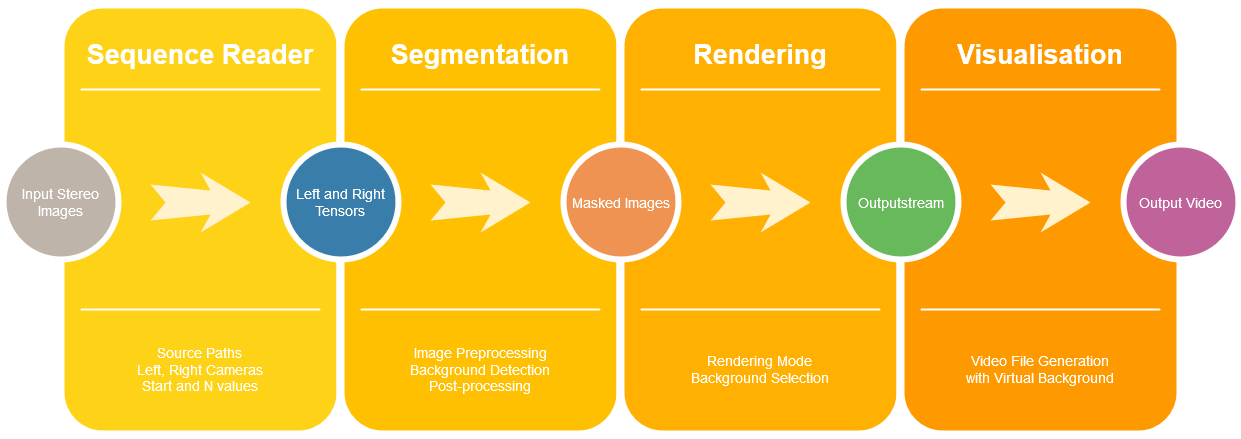
\includegraphics[width=12cm]{overviewConcept}
	\caption{Overview of Concept}
\end{figure}


\subsection{Image Reader}

The extraction of the frames follows the logic represented in figure ~\ref{fig:flowchart}. The user can pick the starting frame for extraction and the total number of frames to load. If the number of loaded frames reaches the end of the available frames, a loop value will be set to one and the next run will automatically start at the first frame of the stream, independently from the start value.
\begin{figure}[!h]
	\centering
	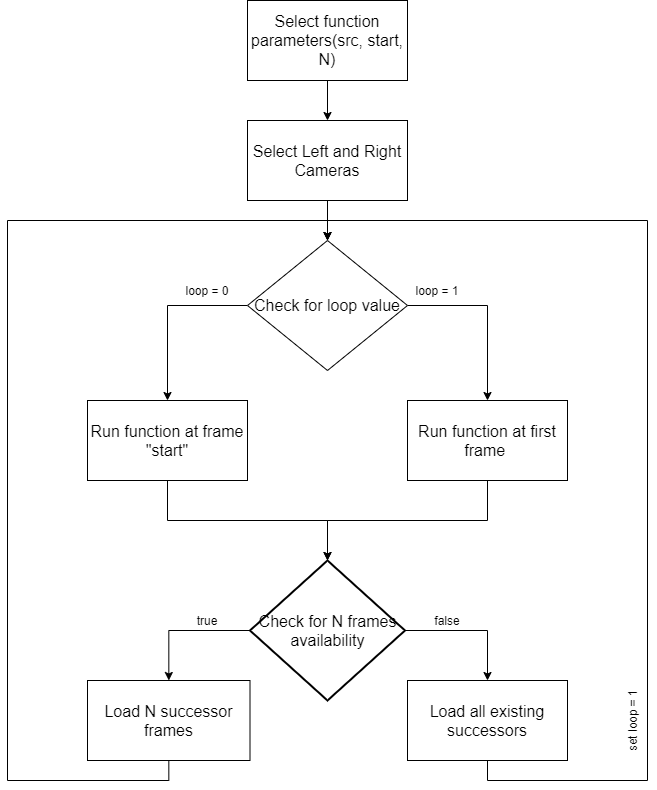
\includegraphics[width=0.9\textwidth]{flowchart}
	\label{fig:flowchart}
\end{figure}
\newpage
First, to read the images we have in each sequence it was important to implement the ImageReader Class which has several input parameters given through the constructor and the method Next which returns N subsequent image pairs starting at the value specified in the parameter start.
\\
Next, as we have multiple views angles from three different cameras it was important to select the two source paths left path and right path (C1 for the first camera, C2 for the second camera, C3 for the third camera) using the variable src and both of properties L and R which identify the cameras. 
\\
Due to the gaps in the images numbers, it was more convenient to extract the images pairwise from the text file which contains all their names. 
\\
As a further step, The variable loop was initialized with 0 and then could be changed to 1 if the reader had reached the end of the path. Depending on its value the method next would either start reading from the beginning of the file or the given start.
\\
This method has three outputs: loop variable for the next call of the function and two tensors ( left tensor for the left camera, right tensor for the right camera )in which the frames of both cameras will be saved.
\subsection{Image Segmentation}
The following Block diagram explains our proposed solution for the segmentation part of the program: 	

\begin{figure}[!h]
	\centering
	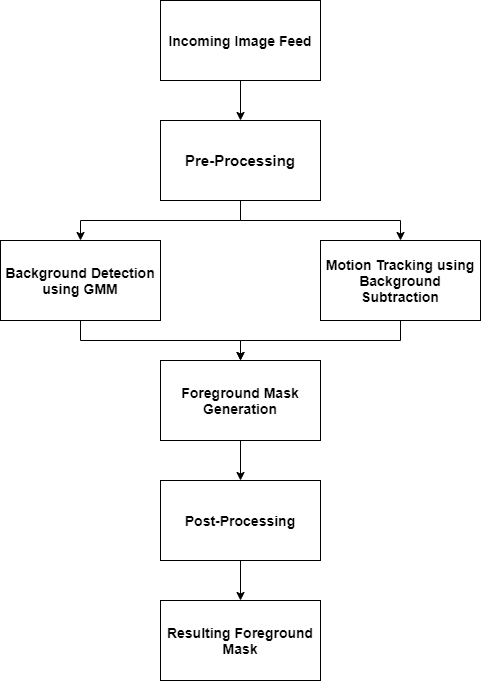
\includegraphics[width=0.9\textwidth]{chart}
	\label{fig:chart}
\end{figure}
\newpage
\subsubsection{Pre-processing}
Pre-processing the incoming image feed is an important step in a computer vision application. The main goal of this phase is to raise the quality of the data either through the enhancement of certain image features or the removal of undesirable ones. Denoising for example could be achieved by using specific filters such as the median filter (especially known for its efficiency against salt and pepper noise) and the low-pass filter. Gaussian blur could also be used as a Gaussian noise reduction technique as well as a means to enhance some image structures.
\\
Another popular technique commonly used in image processing is normalization. This term could refer at the same time to statistical normalization and also luminance normalization. The former stands for the conversion of all images to “normalized” images having 0 as their mean values and 1 as the standard deviation. As for the latter, the process seeks to change the intensity values of the individual pixels in images, this could be achieved using the method of histogram stretching (also known as contrast stretching) to increase contrast or using histogram equalization to enhance it. 
\subsubsection{Foreground Detection using Gaussian Mixtures Models}
The Computer Vision Toolbox available in Matlab provides a ready-to-use foreground detection method using Gaussian mixtures models. The vision.ForegroundDetector function comes with a set of properties that provide a certain degree of freedom during implementation such as the number of Gaussian modes used in the mixture model and the number of frames used for training background model. Another crucial property of the foreground detector is the Initial Variance which depends on the range of pixel values in the image feed. For images with data type ‘double’ or ‘single’, pixel values range between 0 and 1 meaning that the initial variance should be set to \((30/255)^2\)  whereas if the images are loaded as a ‘uint8’ object, then the initial variance takes in a value of \(30^2\).
\\
As the provided dataset is comprised of mostly images taken inside an indoor environment, we use 2 Gaussian modes in the mixture models; this is due to the fact that indoor images have a static background most of the time thus meaning that increasing the number of Gaussian modes (typically applied to model multiple background modes) may lead, in our case, to wrong or inaccurate detections. For the other properties, the algorithm initially loads the first 100 frames to use for training with an adaptative learning rate corresponding to \(1/\left(current\ frame\ number\right)\) . After this initial training, the learning rate is set to 0.01 for the remainder of the foreground detection process leading at the end to the generation of a binary foreground mask. 

\subsubsection{Motion Tracking using Background Subtraction}
The proposed algorithm used in this part aims to estimate moving edge pixels by comparison of two successive masks. These masks are obtained by extracting the background from two images. To do this, we first define a threshold ratio for pixels values. Next, we subtract the previous image from the current one and compare the resulting image to the previous image scaled by the defined threshold value. This would result in a binary mask where pixels that are below the previous image threshold are considered as background and those with greater values are assumed belonging to the foreground. To reduce noise in the mask, we multiply it with the mask generated in the previous run.
\subsubsection{Foreground Mask Generation}
The previous methods presented above output two binary masks that could be used for foreground detection, however, both of the generated masks present wrong detections. On one hand, the foreground detection sometimes identifies parts of the foreground as background and vice-versa. For example, somber clothes are sometimes identified as background when the scene has bleak lighting whereas, in a bright scene, some parts of the background could be identified as foreground if the person(s) is(are) wearing bright clothes. On the other hand, the mask generated in the third step should now indicate the shape of moving objects in the image. As the objective is to consider moving objects as foreground, we draw the boundary of these shapes then fill their insides with white pixels. This method proves however to be challenging when dealing with an image containing 2 or more persons that are distanced from each other. To circumvent these issues, we combine the two masks obtained through the previous techniques to generate the resulting foreground mask which would be passed on to post-processing.     
\subsubsection{Post-Processing}
The resulting mask from the previous phase may still include some unwanted portions that distort the detection. This may arise due to some changes in the background condition and takes the shape of noise or small holes in the mask. To deal with these issues, post-processing techniques are implemented to remove unwanted portions from the foreground mask and “fill” other undetected areas that originally belong to the foreground of the scene. To remove small noisy blobs, noise filtering algorithms are of extreme importance; this step is extremely important and needs to proceed with other post-processing operations as this noisy detection may badly interfere with future operations.  The second half of post-processing implies the changing of shapes of detected blobs to bring them closer to the ground truth. Dilation and erosion are considered to be the most basic morphological operations. After defining the size and shape of the structuring element, dilation expands objects by adding pixels to the boundaries of detected blobs in the image according to the defined structuring element whereas erosion does exactly the opposite by removing pixels.  
\subsection{Image Renderer}
After segmenting the foreground in images, the function rendering can process an image of the left camera frame using its segmented mask according to a chosen mode given as a string. The argument mask is a matrix of a binary image which have the same size as the frame image. The function rendering can be called using one of these modes:
\\
\begin{itemize}
	\item \textbf{foreground:} When calling the function render using the foreground mode the background is set to black and the foreground in the image will be displayed. Since the foreground pixels are ones and the background pixels are zeros in the matrix “mask”, the output is computed by simply performing an element-wise multiplication of the mask and the frame image. By doing so, all background pixels are set to zero and only foreground ones keep their RGB values.
	\item \textbf{background:} When calling the function render using the background mode the foreground is set to black and only the background is displayed. To keep the values of the background pixels and set the foreground pixels to zero, the mask is first inverted so that its element-wise multiplication by the frame image keeps only the RGB background values.
	\item \textbf{overlay:}When calling the function render using the overlay mode foreground and background is displayed with two different colours transparently. For the overlay mode, a copy of the mask is inverted. Each of the masks and the inverted mask matrices is multiplied by two different RGB vectors and summed, then the two 3 dimensional matrices are summed so that the foreground and background are shown with two different colours.
	\item \textbf{substitute:}When calling the function render using the substitute mode the background is replaced with a given virtual background. As the background image should have the same size as the frame image, the virtual background image is resized. To keep the pixel values of the foreground, the frame is element-wise multiplied by the mask matrix, whereas the virtual background is multiplied by the inverted mask. After summing the two RGB images, the existing background is replaced with the virtual background.
\end{itemize}